%!TEX root = ../dissertation.tex

\iffalse \bibliography{bibliography/dissertation} \fi


\chapter{Related Work}
\label{chapter:relatedWork}

In this chapter, I summarize related research on development environments and programming languages. Work presented here focuses on the programming tools used in distinct contexts and situations, whereas Chapter~\ref{chapter:evaluation}  discusses technical aspects and software architecture.

My work lies at the intersection of two main research areas: software engineering (SE) and generative design (GD). Consequently, the related work includes advances in both of these areas.

\section{Programming System}
\label{sec:ps}

A \textit{programming system} has two fundamental parts: the \textit{programming language} that users should know to create a program, and the \textit{programming environment} that is used to write and test programs. Undoubtedly, both parts are equally important to build a program and understand it. However the boundaries between these components can be blurred, for this reason, the related work goes beyond programming environments including also programming languages and their design aspects. 

Based on prior surveys of novice programming environments~\citep{kelleher2005lowering}, in the following sections I divide the programming systems into three categories: (\ref{sec:gs}) general-purpose systems; proposed for building sophisticated software, (\ref{sec:ts}) teaching systems; intended to teach programming, and (\ref{sec:es}) empowering systems; proposed to build programs tailored to specific needs. In each category, I focus on the tools provided by the programming environment.
%%%
\section{General-purpose systems}
\label{sec:gs}

The systems in this category are built to support all, or at least a substantial part, of the software development process. To this end, these systems suggest an \gls{ide} that aims to support the entire development process by grouping in a single environment all necessary tools.

In this section we describe, in detail, two relevant \glspl{ide}: Eclipse~(open-source)~\citep{carlson2005eclipse} and LightTable (open-source)\footnote{\label{fnote:lt}\texttt{http://lighttable.com/}}. Other popular \glspl{ide} include NetBeans~(open-source)~\citep{boudreau2002netbeans}, Microsoft's Visual Studio~(commercial)~\citep{guckenheimer2006software}, or Apple's Xcode~(free but closed-source)\footnote{\texttt{https://developer.apple.com/xcode/}}. Some \glspl{ide} (eg., Visual Studio or Xcode) primarily target the environment and ecosystem of the manufacturer's own programming languages.  The following study use those \glspl{ide} for the sake of comparison, because they provide similar features to Eclipse or LightTable.

%%%%%%%%%%%%%%%%%%%%%%%%%%%%%%%%%%%%%%%%%%%%%%%%%%%%%%%%%%%%%%%%%%%%%%%%%%%%%%%%%%%%%%%%%%%%%%%%%%%%%%%%%
\subsection{Eclipse} 
\label{subsec:eclipse}
Eclipse~(Figure \ref{fig:eclipse}), a project initiated in 2001 and promoted by a consortium of industry leaders~\citep{carlson2005eclipse}, is a widely used open-source \gls{ide}. It is used mainly by Java developers, although it supports additional programming languages such as C, C++, and JavaScript. As showed in~\citep{murphy2006java}, the commonly cited reasons for using Eclipse include rich Java development tools support and a \textit{plugin} architecture, the Eclipse Platform~\citep{DesRivieres2004}, that allows steady integration of third-party functionality.

The Eclipse platform~\citep{DesRivieres2004} has a similar design among the \glspl{ide} presented in this category. This architecture has two main components, the \textit{plugin} which is the smallest unit of functionality that can be developed and delivered separately, and the platform runtime which will discover and connect the \textit{plugins} to the platform itself. As a result, the platform integrates several tools used in distinct phases of the software development process. Figure~\ref{fig:eclipse} shows the \gls{ide} opened in the Java perspective, suggesting a quick fix for the error.

\begin{figure}[!htbp]
%\vspace{-5pt}
  \centering
  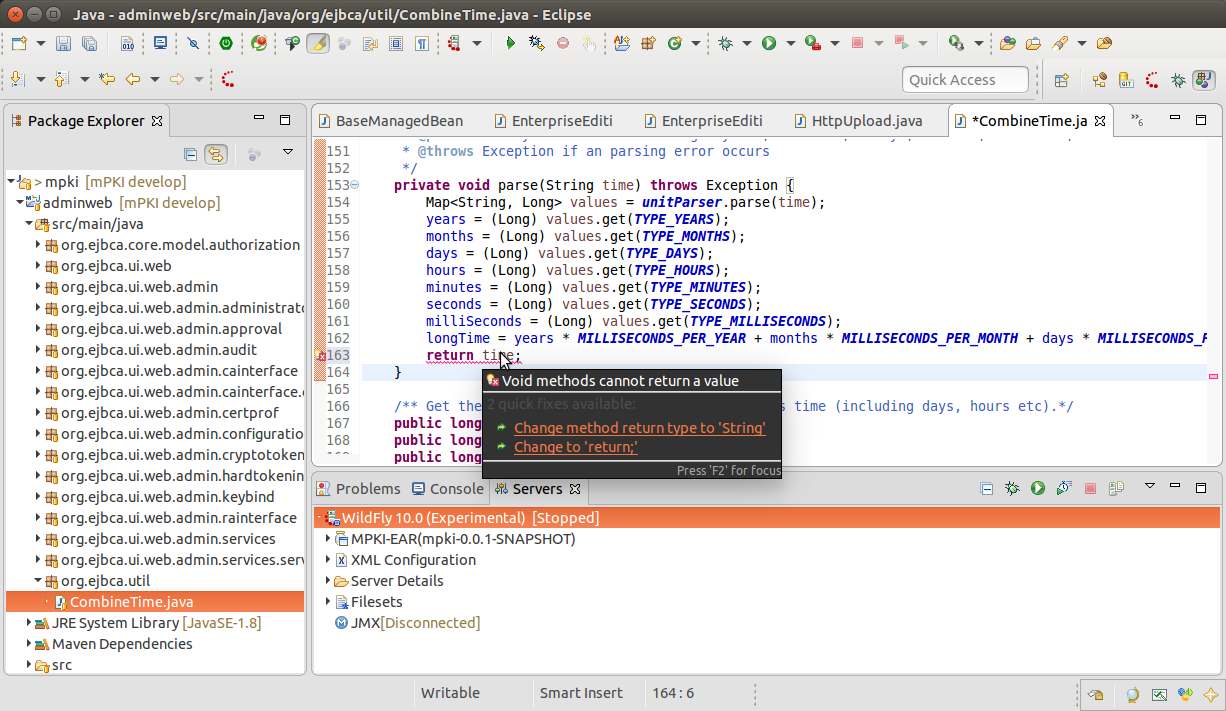
\includegraphics[width=1.0\textwidth]{images/eclipse-2}
    %\vspace{-15pt}
    \caption{Eclipse Integrated Development Environment showing Java perspective}
    %\vspace{-5pt}  
  \label{fig:eclipse}
\end{figure} 

Programming is a laborious task, even worse with a verbose programming language such as Java. For example, while the developer is writing code he usually makes some errors, from lexical errors to semantic errors, that he will only detect after compiling the code. So, he needs to stop his primary task to compile the code and eventually debug it. This edit-compile-debug cycle is unproductive and naturally undesired in an industry environment. 

To prevent this problem, a standard feature among \glspl{ide} is the instant feedback. This feature aims to anticipate the state of the current program by indicating eventual errors or mistakes made during development. To provide instant feedback Eclipse is always compiling the code in the background, and giving immediate feedback for the developer in the form of syntax highlighting, code completion suggestions, and indications of problems associated with various locations in a source file. 

In the literature a similar concept, known as \textit{liveness}~\citep{alpern1985defining}, referring to the ability to modify a running program. There are several levels of liveness, and this kind of tool represent the first level~\citep{tanimoto2013perspective}. The tools in the first levels respond after an action while the tools at the last level not only run the program and respond immediately but also predict the next programmer action. Having those tools in a \gls{ide} would be the ideal. However, it is far from the reality of nowadays \glspl{ide} tools. 

Before to idealize new features is important to highlight the drawbacks of the existent ones. Eclipse, as the others similar \glspl{ide}, share some problems, as for instance:

\begin{itemize}
    \item They are incidentally complex. There is an immense amount of work to be done in those \glspl{ide} that is indirectly related to the real problem itself. For example, until the developer gets a simple program to run, he needs to install, configure a set of necessary software, and he also needs to set up the development environment. These are tiresome and time-consuming tasks that add extra complexity to programming which is already a complicated subject.

    \item Program execution is hard to observe, such that the only way to see how the program executes is by a stepwise debugger. This process forces the programmer to stop the program and look at a line in a single instant of time. Therefore, the programmer cannot see how his program is executing, nor how his changes affect its execution.
\end{itemize}

The complexity of install and configure an \gls{ide} negatively affects the programming language itself, because users are more interested in the capabilities of the language than the \gls{ide}. To overcome this problem, recent programming languages, such as Rust~\citep{matsakis2014rust}, propose an \gls{ide} on the web browser\footnote{\texttt{https://play.rust-lang.org/}}. So users can write programs and use the language without any previous configuration. However this web environment is suitable only for tutorials and small examples, otherwise to have full access to the language users must pay the price to install and configure the language and the \gls{ide}.

%%%%%%%%%%%%%%%%%%%%%%%%%%%%%%%%%%%%%%%%%%%%%%%%%%%%%%%%%%%%%%%%%%%%%%%%%%%%%%%%%%%%%%%%%%%%%%%%%%%%%%%%%
\subsection{LightTable}
\label{subsec:lighttable}
LightTable$^{\ref{fnote:lt}}$ is a successfully crowd-funded project that indicates that instant feedback attracts wide interest beyond the research community. Similarly, Apple has recently integrated a feature called Playgrounds into the Xcode \gls{ide}. Playgrounds are enabled by Apple's new programming language Swift\footnote{\texttt{https://developer.apple.com/swift/}} and allow developers to edit code and immediately see the results of the execution.

LightTable is based on Bret Victor ideas which in his influential work~\citep{inventingPrin,learnableProg} pointed out serious problems with the current environments and showed, using prototypes, how the environment can help to address those problems. LighTable is proposed to build web application, to support this process, it provides, at least, two useful features: (1) live execution feedback, that executes the program on every change showing the program flow, and (2) the organization of code in tables, enabling quick access to the program documentation.

\begin{figure}[!htbp]
%\vspace{-10pt}
  \centering
  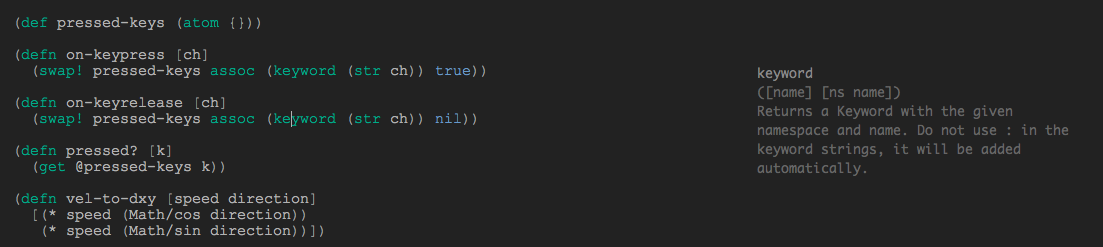
\includegraphics[width=1.0\textwidth]{images/lt2}
    %\vspace{-15pt}
    \caption{LighTable interactive development environment}
    %\vspace{-10pt}  
  \label{fig:lt}
\end{figure} 

LightTable was initially implemented in Clojure\footnote{\texttt{https://clojure.org/}} a general-purpose programming language dialect of Lisp that runs on top of \gls{jvm}. Progressively the code originally written in Clojure was rewritten in ClojureScript\footnote{\texttt{http://clojure.org/clojurescript}}, a scripting language that uses Clojure compiler which targets JavaScript. Due to its implementation, in LightTable adding a new \gls{ui} element into the programming environment or changing an existing one is doable in a short amount of time, contrary to other \glspl{ide}, such as Eclipse~\citep{carlson2005eclipse}, where an equivalent change requires considerable amounts of time. 

LightTable provides a lateral panel for ease documentation access so that users can read any primitive functions of Clojure or ClojureScript. This documentation is a textual description of the function parameters, the type of return, and some usage suggestions. While looking at a program, it is helpful to have the documentation of strange primitives, such as the \texttt{keyword} function, shown in Figure~\ref{fig:lt}, however, non-primitive functions are still undocumented. 

\begin{wrapfigure}{r}{0.3\textwidth}
  %\vspace{-30pt}
  \begin{center}
    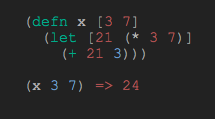
\includegraphics[width=0.3\textwidth]{images/eval-close}
  \end{center}
  %\vspace{-15pt}
 \caption{LightTable real-time debugger.}  
  %\vspace{-20pt}
    \label{fig:lt2}
\end{wrapfigure}

On the other hand, programmers are encouraged to understand new functions by seeing how the values of a function call flow through it. This feature is based on the old idea of Lisp environments: the \gls{repl} which is a prompt used to try out expressions of the language without having to run all the code. This approach goes further by using reflection mechanisms to trace the function call values and shows them filled in the function template (as shown in Figure~\ref{fig:lt2} the flow of values produced by calling \texttt{(x 3 7)}).

The real-time debugger is an interactive way to debug the code and understand the program flow. Using this feature in an arbitrarily complex program (a program with more than 30 functions) is, however, worthless, because, all the programmer sees is a replica of his functions filled with numbers. It is a poor representation of flow which forces the developers to spend as much effort on this feature as without it. For this reason, other systems, described in this report, represent the program flow using graphs which are more appropriate in some cases, for example, to show error occurrences in the source code.

Despite providing some tools which are state of the art, LightTable remains in an experimental phase. It has severe limitations to identify and clearly present the errors in the source code. This problem is, mainly, related with the Clojure compiler which loses significant \textit{metadata} between conversions. Consequently, programmers can spend more time and effort to find a bug using LighTable, than using the other \glspl{ide}, such as Eclipse.
%%%%%%%%%%%%%%%%%%%%%%%%%%%%%%%%%%%%%%%%%%%%%%%%%%%%%%%%%%%%%%%%%%%%%%%%%%%%%%%%%%%%%%%%%%%%%%%%%%%%%%%%%
\section{Teaching systems}
\label{sec:ts}
Unlike the previous systems, teaching systems are designed with the goal of helping people learning to program. Most of the systems in this category provide simple programming tools that expose the novice programmers some of the fundamental aspects of the programming process. After acquiring experience with a teaching system, students are expected to move to a more general-purpose environment. 

%%%%%%%%%%%%%%%%%%%%%%%%%%%%%%%%%%%%%%%%%%%%%%%%%%%%%%%%%%%%%%%%%%%%%%%%%%%%%%%%%%%%%%%%%%%%%%%%%%%%%%%%%
\subsection{LOGO} 
\label{subsec:logo}
LOGO~\citep{papert1980mindstorms} is a programming language and environment intended to allow children to explore a wide variety of topics such as physics and mathematics. The programming language is a dialect of Lisp, with much of the punctuation removed to make the syntax accessible to children, it uses a helpful metaphor which facilitates the introduction of programming concepts.

In Logo, the novice programmers draw pictures by directing the ``turtle'', an onscreen character which leaves a trail as it moves (see Figure~\ref{fig:turtle}). The turtle is a metaphor that helps learners to translate their experiences as a person into programming knowledge. That means, to figure out how to make the turtle perform an action, the programmer can ask how he would perform that action himself as if he were the turtle.

\begin{wrapfigure}{r}{0.4\textwidth}
  %\vspace{-40pt}
  \begin{center}
    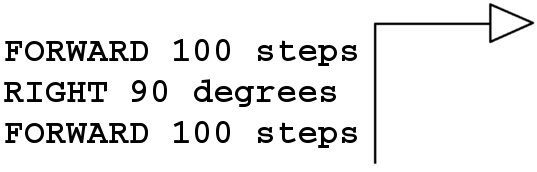
\includegraphics[width=0.4\textwidth]{images/turtle}
  \end{center}
  %\vspace{-15pt}
 \caption{Directing the ``turtle''.}  
  %\vspace{-20pt}
    \label{fig:turtle}
\end{wrapfigure}

For example, to figure out how to draw a circle, a learner would walk around in circles for a bit, and quickly derive a ``circle procedure'' of taking a step forward, turning a bit, taking another step forward, turning a bit. After teaching it to himself, the learner can then teach it to the computer. 

LOGO has influenced several systems, and its principles show how a system can be designed around the way people think and learn.
%%%%%%%%%%%%%%%%%%%%%%%%%%%%%%%%%%%%%%%%%%%%%%%%%%%%%%%%%%%%%%%%%%%%%%%%%%%%%%%%%%%%%%%%%%%%%%%%%%%%%%%%%
\subsection{SmallTalk}
\label{subsec:smalltalk}
SmallTalk~\citep{Kay1993} is a programming language and environment to support children in the world of information. The designers of this system wanted to create a programming language that had a simple model of execution, and a programming methodology that could accommodate a wide variety of programming styles. SmallTalk was based on three ideas: (1) everything is an object, (2) objects have memory in the form of other objects,  and (3)objects can communicate with each other through messages.

\begin{wrapfigure}{r}{0.5\textwidth}
%\vspace{-20pt}
  \centering
  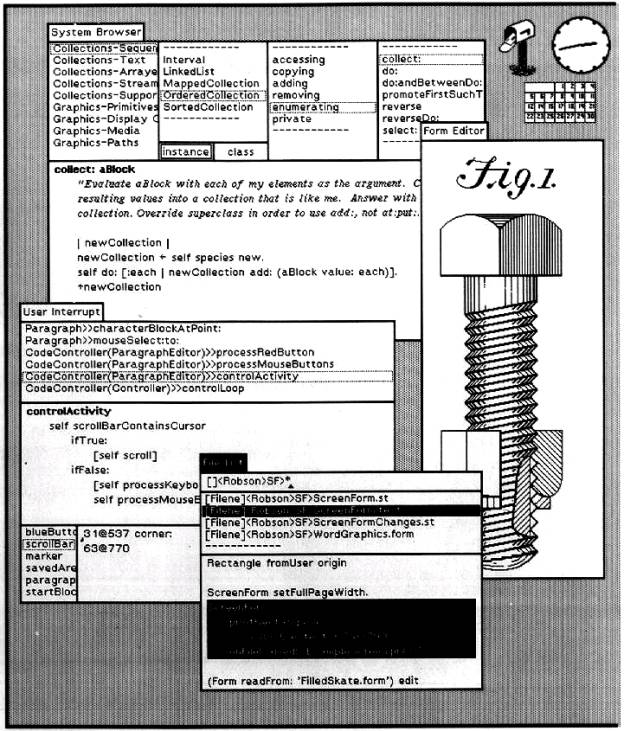
\includegraphics[width=0.5\textwidth]{images/smalltalk}
    %\vspace{-15pt}
    \caption{Smalltalk user interface.}
    \vspace{-20pt}  
  \label{fig:smalltalk}
\end{wrapfigure} 

Smalltalk programming environment was an achievement with consistent improvements on its successors. The system consisted of about 50 classes described in about 180 pages of source code~\citep{Kay1993}. This included all of the OS functions, files, printing and other Ethernet services, the window interface, editors, graphics and painting systems, as shown in Figure~\ref{fig:smalltalk}. 

In the Smalltalk programming language, the communication through messages has a strong resonant metaphor. To specify the behavior of an object, the programmer casts himself into the role of that object (to the extent of referring to the object as ``self'') and thinks of himself as carrying on a conversation with other objects. This is a strong metaphor because role-playing and conversing are innate human facilities. 

In fact, SmallTalk features are, nowadays, a consistent reference for any programming system.
%%%%%%%%%%%%%%%%%%%%%%%%%%%%%%%%%%%%%%%%%%%%%%%%%%%%%%%%%%%%%%%%%%%%%%%%%%%%%%%%%%%%%%%%%%%%%%%%%%%%%%%%%
\subsection{Processing}
\label{subsec:processing}
Processing~\citep{Reas2006} is a programming language and environment designed to teach programming in an optic context. Processing has become popular among students, artists, designers, and architects because it acts as a tool to get non-programmers started with programming through instant visual feedback.

The Processing programming language is built on top of Java, but it removes much of the verbosity of Java to make the syntax accessible to novices. The language provides simple access to external libraries, such as OpenGL, through single entry points, such as \texttt{setup} and \texttt{draw}. Therefore, this allows novices to quickly prototype, learn fundamental concepts of programming, and, eventually, gain the basis to learn other programming languages.

The programming environment contains a simple text editor, a text console to present errors, and a run button. The run button compiles the Processing code and executes it. Moreover, in the default mode, the program result is displayed in a 2D graphical window, the render can be configured to present the result in 3D, or other sophisticated methods using \textit{shaders} to recur directly to the graphic board.

Actually, with a few changes, the Processing code can be exported as an application for different platforms, such as Java, JavaScript, and Android. For example, to export a Processing program for JavaScript, it is only necessary to create a HTML page and include the Processing code as a script of this page. Then the Processing code will be automatically parsed and translated to JavaScript. To maintain the usual render capabilities of a Processing program, it will use the HMTL5 canvas with WebGL.

The popularity of Processing is explained by the benefits of these features, besides of being a domain-specific language. However, it has drawbacks that can discourage its use, such as the following:

\begin{itemize}
  \item \textit{Weak metaphor}. The Processing programming language, by contrast with the above systems, has none strong metaphors that allow the programmer to translate his experiences as a person into programming knowledge. 

  \item \textit{Poor decomposition}. Processing discourages the elementary approach to solving a complex problem by breaking it into simpler problems because drawing and input events link to single entry points. Thereby the behavior of submodules must be tangled across these global functions, making it difficult to achieve clean decomposition.

  \item \textit{Poor recomposition}. Processing discourages combining two programs. The designer cannot just grab and use part of other programs because variables must be renamed or manually encapsulated, and the \texttt{draw} and mouse functions must be woven together. Even worse, Processing has global modes which alter the meaning of the function arguments. For example, two Processing programs can specify its colors in different modes and each mode has its proper purpose of \texttt{fill} function arguments. Combining those programs will be almost impossible. 

  \item \textit{Weak readability}. The syntax of a Processing program represents a significant barrier for reading. For example, the function which draws an ellipse on screen is written as \texttt{ellipse(50,50,100,100)}. The reader must look up or memorize the meaning of every single argument.

  \item \textit{Fragile environment}. The programming environment is fragile because it does not attempt to solve any of the above issues related to the language and its implementation.
\end{itemize}

%%%%%%%%%%%%%%%%%%%%%%%%%%%%%%%%%%%%%%%%%%%%%%%%%%%%%%%%%%%%%%%%%%%%%%%%%%%%%%%%%%%%%%%%%%%%%%%%%%%%%%%%%
\subsection{Fluxus}
\label{subsec:fluxus}
Fluxus~\citep{griffiths2007fluxus}\footnote{\texttt{http://www.pawfal.org/fluxus/}} is a programming language and learning environment designed for rapid prototype using 3D graphics and sounds. This emphasis on the primitive prototype and instantaneous feedback makes Fluxus a tool for learning computer animation, graphics, and programming. However, most users of Fluxus use it for \textit{livecoding}, which is the act of performing coding lively to an audience.

Fluxus is mainly written in C++, and it links statically to several shared libraries, specified at compile time. For instance, Fluxus uses \texttt{jack-audio}, \texttt{ode}, and \texttt{fftw} libraries to handle and synchronize the audio, \texttt{GLEW} to present graphics, and \texttt{racket3m} to embed the Racket run-time system into the application. In this way, Fluxus is an extension of Racket (a descendant of Scheme) with graphical commands.

Like Processing, Fluxus provides direct access to those libraries through single entry points, for instance, \texttt{start-audio} connects an input audio to the application, \texttt{every-frame} registers a function called once per frame, and so on. However, as stated above, it is a barrier for decomposition since the behavior of submodules must be tangled across these global functions.

\begin{figure}[!htbp]
  \centering
  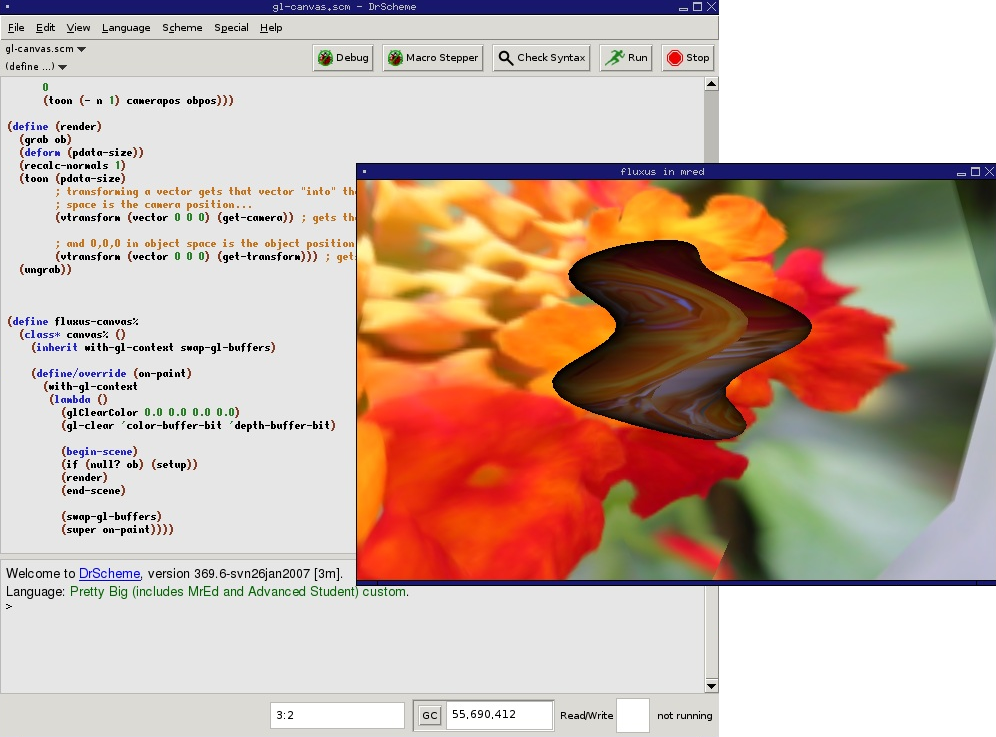
\includegraphics[width=.8\textwidth]{images/fluxus}
    \caption{Fluxus engine being used as DrRacket module}
  \label{fig:fluxus}
\end{figure} 

Fluxus has its environment specifically tailored for \textit{livecoding}. It has a OpenGL graphical window with a simple text editor. The performer types his code in the editor and presses a shortcut key each time he wants to run it. Fluxus evaluates the code through Racket run-time system, showing the result in the same graphical window, also used as a text editor. This mechanism is valuable in a \textit{livecoding} environment, because the performer can be editing the code while maintaining at the background, the result of the previous computation. However, if the code has any error and the performer execute it, the previous calculation disappears, and the environment will not help to find it. In fact, this is a serious problem, especially for the Racket syntax.

Moreover, Fluxus shares with Processing similar drawbacks to those previously stated. However, Fluxus can be used as a module of DrRacket (Figure~\ref{fig:fluxus})~\citep{findler2002drscheme} programming environment. Fortunately, DrRacket solves the above problem and many others.
%%%%%%%%%%%%%%%%%%%%%%%%%%%%%%%%%%%%%%%%%%%%%%%%%%%%%%%%%%%%%%%%%%%%%%%%%%%%%%%%%%%%%%%%%%%%%%%%%%%%%%%%%
\subsection{DrRacket}
\label{subsec:drracket}
DrRacket~\citep{findler2002drscheme} is a programming environment designed to support the Racket language. DrRacket is one of few programming environments which supports continuous learning in a more general language from the start. Consequently, it has been widely used in introductory programming courses in several universities around the world.

DrRacket is usually used to introduce the fundamentals of programming. To facilitate this process, DrRacket provides three tools. The first is a symbolic stepper. It models the execution of Racket programs as algebraic reductions, once Racket is implemented on top of lambda calculus. The second tool is a syntax checker. It annotates programs with font and color changes based on the syntactic structure of the program. It also permits students to explore the lexical structure of their programs graphically and to $\alpha$-rename identifiers. The third tool is a static debugger that infers which set of values an expression may produce and how values flow from place to place in the source text, and, upon demand, it explains the reason of errors by drawing value flow graphs over the program text.

Similar to Lisp environments, DrRacket provides a read-eval-print loop (\gls{repl}). A command prompt intended to evaluate expressions quickly and print their results. Particularly in a learning environment, this feature makes an important connection between program execution and algebraic expression evaluation. However, the Lisp-style syntax obscures the effect of this feature. To overcome this limitation, DrRacket provides a \texttt{pretty-printer}. A module capable of printing algebraic expressions in a meaningful way, as well as other graphics elements supported by the text editor, such as images, snips, XML boxes, and so on.

More recently, DrRacket has included picture boxes for \gls{wysiwyg} layout of slide content that is otherwise created programmatically~\citep{findler2004slideshow}. This kind of presentation extensibility is in addition to recognizing standard Racket hygienic macros. There are several problems with this approach. First, there is no documented protocol for creating new kinds of boxes. Second, programs that use media-rich elements are stored as an ASCII-encoded binary which is hard to edit outside DrRacket editor. Last, the semantics of the boxes is driven off of the display itself, rather than the persistent store; therefore, to compile, interpret, or edit the program, a box-aware editor is required.

From the perspective of professional developers, DrRacket can be a potential target. It is useful for developing complex applications, including DrRacket itself. Moreover, it is extensible by the same \gls{api} which the above tools implement. Through this \gls{api} it is also possible to extend the \gls{repl}, as in Pict3D\footnote{\texttt{https://github.com/ntoronto/pict3d}} (a 3D engine that integrates new graphical elements in the DrRacket environment). On the other hand, for supporting extensions, DrRacket's architecture has become increasingly complex. For instance, to make a simple change in an editor's element the developer should be able to understand several modules, unrelated with the problem itself. This extra complexity is a negative impact when DrRacket is chosen as the basis for new development tools.

Despite the identified advantages, DrRacket has some barriers that may discourage the learner. For example, the Racket programming language is simple to teach, but its heavy syntax of s-expressions hinders the student to read the program. Consequently, the learner can spend a considerable mental effort to understand insignificant details of the language.
%%%%%%%%%%%%%%%%%%%%%%%%%%%%%%%%%%%%%%%%%%%%%%%%%%%%%%%%%%%%%%%%%%%%%%%%%%%%%%%%%%%%%%%%%%%%%%%%%%%%%%%%%
\subsection{PythonTutor}
\label{subsec:pythontutor}
PythonTutor~\citep{GuoSIGCSE2013} is a web-based program visualization tool, designed to explain how a piece of Python code executes. It has become popular among students from introductory Computer Science courses. Using this tool, teachers and students can write Python programs directly in the web browser and navigate step by step throughout its execution, seeing the run-time state of data structures.

PyhtonTutor has two main modules: the \textit{backend} which implements the core tool functionality, and the \textit{frontend} which presents the visualization of program's data structures. The \textit{backend} executes the input program under the supervision of the standard Python debugger module (\texttt{bdb}) which stops execution after every executed line and records the program's run-time state. After execution terminates, the \textit{backend} encodes the program state in JSON format, serializing Python data types into native JSON types with extra \textit{metadata} tags and sends it to the \textit{frontend}. The frontend renders the objects using standard web technologies: HTML, CSS, and JavaScript. In this way, users can use the tool without installing any extensions or plugins.

A major concern in PythonTutor is security because the PythonTutor's \textit{backend} executes untrusted Python code from the web. To prevent the execution of dangerous constructs such as {\tt eval}, {\tt exec} and {\tt file I/O}, PythonTutor implements sandboxing. It denies the use of most module imports, by parsing the user's code importing, a strict approach, but effective in this case.

The PythonTutor tool allows the programmer to follow the program execution over time, but he only sees a single point in time at any instant. There is no visual context at all. The entire program flow shows disconnected points in time. For example, the programmer who wants to understand a conditional algorithm, using this tool will not see the pattern of this algorithm neither read it at a higher level.
%%%%%%%%%%%%%%%%%%%%%%%%%%%%%%%%%%%%%%%%%%%%%%%%%%%%%%%%%%%%%%%%%%%%%%%%%%%%%%%%%%%%%%%%%%%%%%%%%%%%%%%%%
\subsection{YinYang}
\label{subsec:yinyang}
YinYang~\citep{mcdirmid2013usable} is a prototype of a programming language and environment whose main feature is the live execution feedback. That means it combines editing and debugging, where updated debug results are conveniently visible while editing. YingYang addresses the above issue in two ways. First, just like the previous system, it allows programmers to see single points of execution directly within the code editor (probe; precede expressions with \texttt{@} operator). Second, it has a pane aside the editor which traces execution with entries that are navigable (trace; print-like statements). Basically, the trace is an enhanced display function which, combined with ``probes'', allows the state of previous executions to be restored. So, programmers can take in the entire program flow at a glance and navigate trough it using probes.

YingYang uses an incremental framework as the basis of its programming model. This framework decomposes the program execution into a tree of nodes that can be re-executed independently on code or input change. However, this decomposition cannot be performed transparently. It requires programmers to specify how to decompose the program. To accomplish this task, one must genuinely understand the granularity and modularity characteristics of the computations being performed by the program. Otherwise changes can sometimes have an immense impact on program re-execution time ($\sim$50ms). Consequently, live programming would actually reduce programmer productivity as developers wait for slow feedback.

Although YinYang provides usable features for a learning environment, such as the live execution feedback, it does not have a suitable language for beginners. The language is merely experimental, and to navigate through the program execution, developers must include probes in the code. At the end of experimentation, the code is full of useless expressions.

%%%%%%%%%%%%%%%%%%%%%%%%%%%%%%%%%%%%%%%%%%%%%%%%%%%%%%%%%%%%%%%%%%%%%%%%%%%%%%%%%%%%%%%%%%%%%%%%%%%%%%%%%
\section{Empowering Systems}
\label{sec:es}
In this category of systems, the most important aspect is to allow people to build programs tailored to their needs. In this section, I describe how systems from two distinct areas are adapted to achieve their user's needs. 

First, I consider Architecture, where new programming languages and environments are being proposed to support the increasing use of \gls{gd}~\citep{mccormack2004generative}. \gls{gd} is a design method that uses algorithms to generate architectural models. Usually, these models are rendered using a \gls{cad} tool. 

Second, I consider Mathematics, where advanced technologies are used to approximate as much as possible the mathematical models to the ones that we can see and understand.

%%%%%%%%%%%%%%%%%%%%%%%%%%%%%%%%%%%%%%%%%%%%%%%%%%%%%%%%%%%%%%%%%%%%%%%%%%%%%%%%%%%%%%%%%%%%%%%%%%%%%%%%%
\subsection{DesignScript}
\label{subsec:designscript}
DesignScript~\citep{aish2012designscript} is a programming language and environment designed to support \gls{gd} with textual methods. It is mainly used by architects and designers to generate geometric models using a script. Then when the script executes it creates new models in a \gls{cad} tool. DesignScript is an AutoDesk\footnote{\texttt{http://www.autodesk.com/products}} product initially proposed to be used within AutoCAD (as shown in Figure~\ref{fig:ds}), nowadays it provides the same functionality on top of Revit, another AutoDesk product used for \gls{bim}. In short, a \gls{bim} model is similar to a \gls{cad} model, but it covers more than just geometry. It also includes spatial relationships, properties of building components, such as manufacturers' details.

\begin{figure}[!htbp]
%\vspace{-5pt}
  \centering
  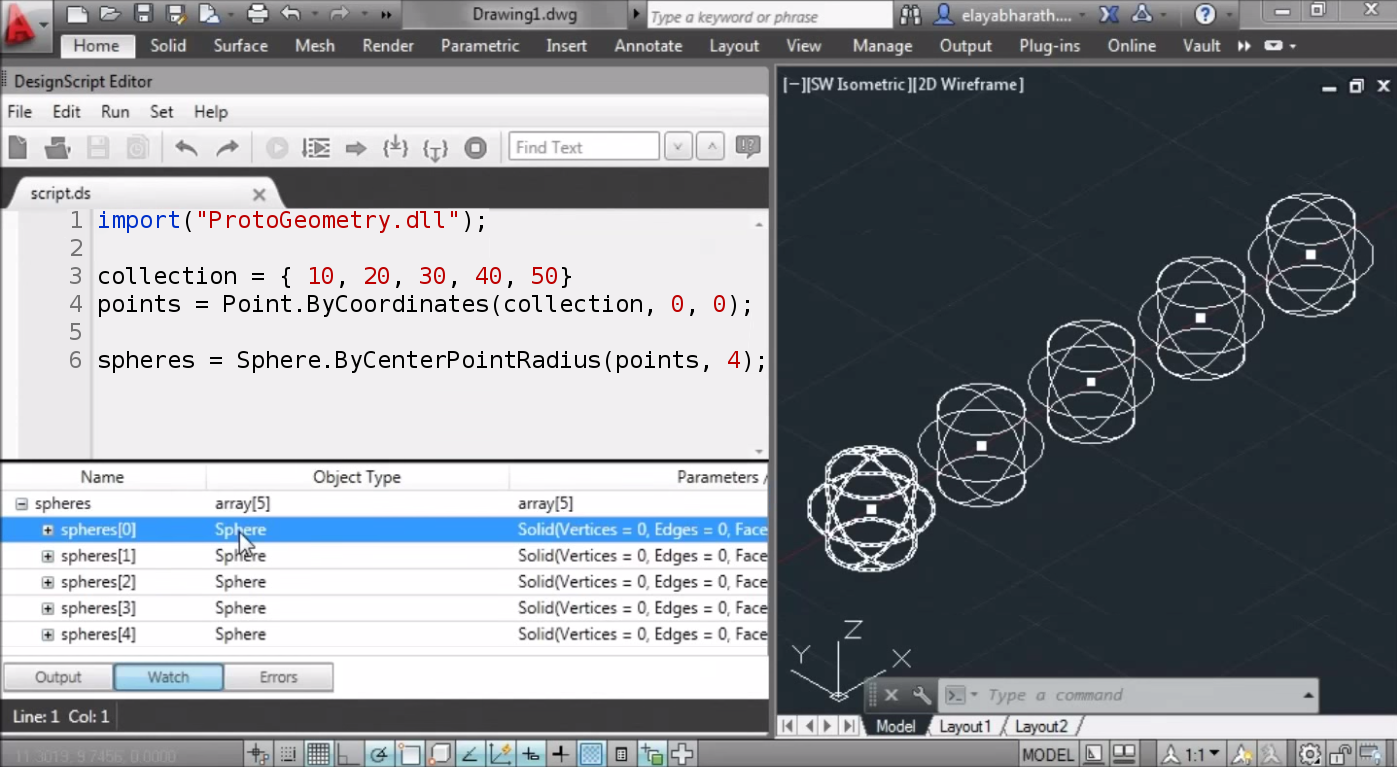
\includegraphics[width=1.0\textwidth]{images/designScriptIDE}
 % \vspace{-15pt}
    \caption{Typical DesignScript programming environment} 
  %  \vspace{-10pt} 
  \label{fig:ds}
\end{figure} 

The programming language is an associative paradigm. The variables are abstract types that can represent numeric values or geometric entities. These variables are in a graph of dependencies. When a change in a variable occurs it forces the re-evaluation of the graph, as shown in Figure~\ref{fig:designscript}, consequently variables has always updated values. This feature is useful, especially in a modeling environment, because it provides continuous feedback to the designer as the model is modified.

\begin{wrapfigure}{r}{0.45\textwidth}
  %\vspace{-5pt}
  \begin{center}
    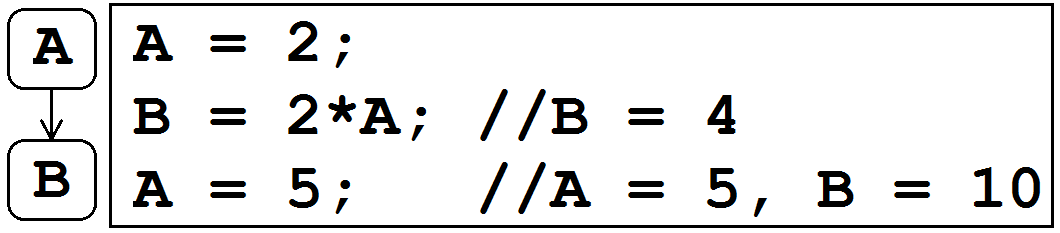
\includegraphics[width=0.45\textwidth]{images/designscript}
  \end{center}
  %\vspace{-20pt}
 \caption{Associative interpretation}  
  %\vspace{-20pt}
    \label{fig:designscript}
\end{wrapfigure}

The DesignScript's programming environment provides a text editor, an interpreter, and a simple debugger. The language interpreter executes each time that the designer clicks on the run button. Then all the script is interpreted, and its result produces geometric entities rendered in the \gls{cad}. The continuous feedback feature works only in debug mode because, in this way, the script is interpreted line by line. Thus, each update to a variable will change its dependencies and will recompute the model. However, in debug mode the code cannot be edited, so this feature is worthless during code editing.

In the DesignScript's debug mode, users can inspect the variable values by adding \textit{watchers} to them. A watched variable is showed in a particular tab, as shown in Figure~\ref{fig:designscript}. In case the variable represents a geometric model, the own design will be highlighted in the \gls{cad} when the variable is selected. It creates a certain \textit{traceability} between patterns in the \gls{cad} and code in the editor. In this way, the user is able to correlate which model a variable corresponds. However the inverse, starting to form the model and finding the correspondent variable, is unsupported.

DesignScript also supports a typical mechanism of \textit{live} programming environments: the sliders. The sliders are widgets which facilitate giving new values to the program input. This way, designers can create new models reacting to these changes. However, in the DesignScript's sliders, the changes are reflected in the models only when the programmer leaves the slider. Until then, the designer should imagine how the model would be with the new value, which is completely against the purpose of sliders.

Moreover the DesignScript language, despite being presented as pedagogic, has some drawbacks. It does not carry any manly metaphor which helps beginners start with the language. Additionally, the associative paradigm represents a barrier for sharing code: it discourages the recomposition of modules because new modules can change the previous one. The environment provides poor mechanisms that help people to find bugs in the code, and finally,  DesignScript is confined to produce geometry in a single \gls{cad} tool.
%%%%%%%%%%%%%%%%%%%%%%%%%%%%%%%%%%%%%%%%%%%%%%%%%%%%%%%%%%%%%%%%%%%%%%%%%%%%%%%%%%%%%%%%%%%%%%%%%%%%%%%%%
\subsection{Monkey} 
\label{subsec:monkey}
Monkey\footnote{\texttt{http://wiki.mcneel.com/developer/monkeyforrhino4}} is a programming environment designed to support \gls{gd}. Like DesignScript, Monkey is used to edit, debug and interpreter scripts. However, Monkey uses RhinoScript as its programming language and Rhinoceros3D\footnote{\label{fnote:rhin}\texttt{https://www.rhino3d.com}} (or Rhino for short), a lighter \gls{cad} than AutoCAD, to generate the geometric models.

Monkey is implemented as a \texttt{.NET} plugin for Rhino4 and provides a programming environment to write and debug scripts. The RhinoScript is based on Microsoft's VBScript language (a descendant of BASIC), and like VBScript, it is a weakly typed language. One of the major drawback with this language is the fact that users must beware with the data passed in their functions at all time because RhinoScript can accidentally cast variables into inappropriate types. Therefore, it creates errors difficult to find, especially for people who are learning to program.

Monkey is based on general-purpose programming environments. It provides typical features of those environments, namely syntax highlighting, auto-completion, and error highlighting. The organization of code into trees is also similar. However, the programming environment and language do not provide any well-designed feature which helps beginners to start with programming. The offered features are based on general-purpose systems, instead of being tailored for \gls{gd}.
%%%%%%%%%%%%%%%%%%%%%%%%%%%%%%%%%%%%%%%%%%%%%%%%%%%%%%%%%%%%%%%%%%%%%%%%%%%%%%%%%%%%%%%%%%%%%%%%%%%%%%%%%
\subsection{Rosetta}
\label{subsec:rosetta}
Rosetta~\citep{lopes2011portable} is a programming environment designed to support \gls{gd} that is based on DrRacket~\citep{findler2002drscheme}. Like Monkey, Rosetta provides its environment detached from the \gls{cad}. Rosetta is a step forward from the previous systems, because it solves the portability problem among \gls{cad} tools. In Rosetta a \gls{gd} program can be written in various programming languages (frontends) and the geometric models can be rendered by different \glspl{cad} (backends). As a result, designers are free to write their programs in their selected frontend which, upon execution, will generate the same geometry for the various backends. In Figure~\ref{fig:rosetta}, a program is written in Racket, and its execution produces geometry for AutoCAD.

\begin{figure}[!htbp]
%\vspace{-5pt}
  \centering
  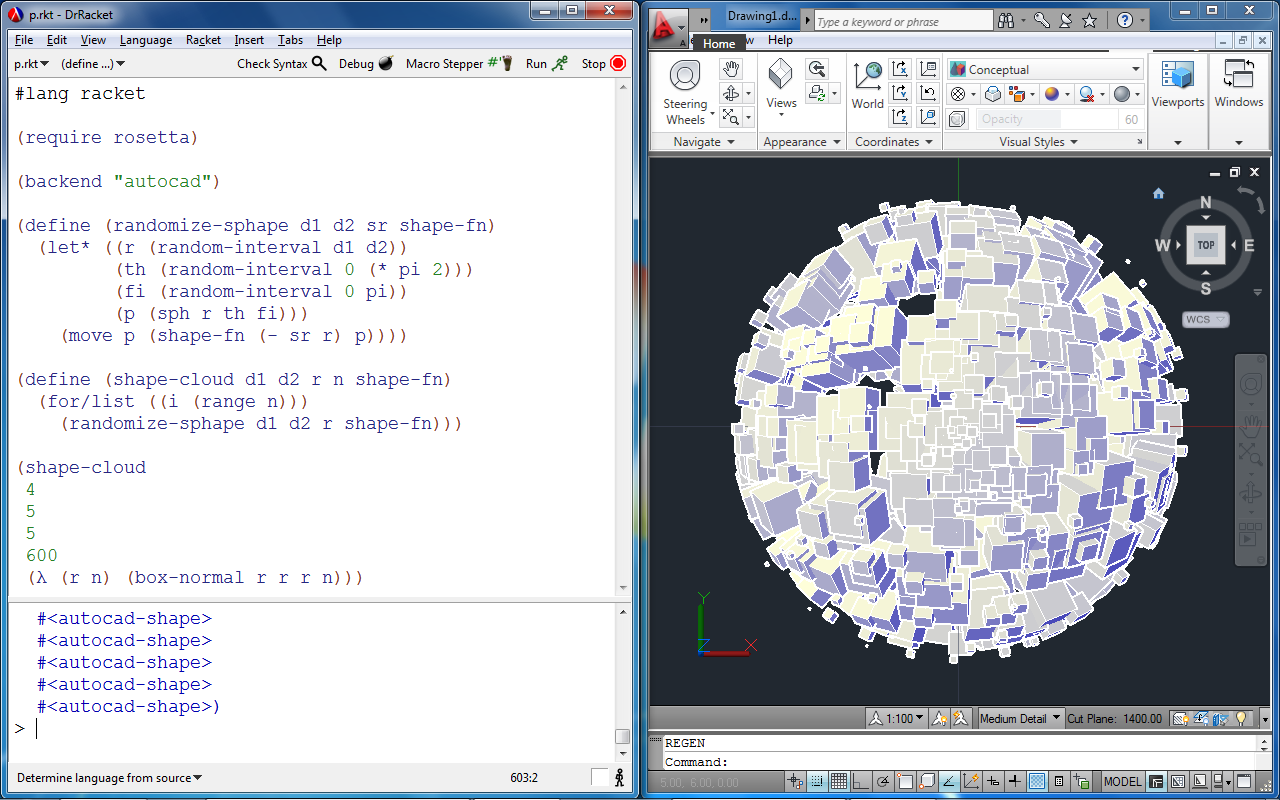
\includegraphics[width=1.0\textwidth]{images/rosetta1}
  %\vspace{-20pt}
    \caption{Rosetta programming environment.}  
  \label{fig:rosetta}
  %\vspace{-10pt}
\end{figure} 

Rosetta has been used to teach programming in architecture courses. Tailored to this end, Rosetta uses DrRacketas its programming environment. The DrRacket environment serves some functions, but the most important are that the student can start immediately to learn to program. For instance, the environment is set up with just three lines of code. As shown in Figure~\ref{fig:rosetta}, the \texttt{\#lang} specifies the frontend language, the \texttt{require} imports Rosetta's primitives and finally the \texttt{backend} names a possible backend.

The Racket language is also an advantage of Rosetta's environment because it encourages the use of the scientific paradigm for writing algorithms. In this way, students that learn simple programming techniques, such as recursion, can create robust models. Additionally, as the students progress, new programming languages are also available to learn, such as JavaScript, Python, Processing, and so on.

The Rosetta's environment provides some interesting tools for \gls{gd}, such as a programming flow tracer, similar to the DesignScript's watcher. It highlights models in the \gls{cad} upon selection of expressions, it also supports the inverse, selecting the mode in the \gls{cad} and shows the expression in the code editor. Another interactive tool is the slider, an attempt to provide immediate feedback to the designers. It uses the DrRacket slider, associating the slider callback to the function that generates the entire model, so each time the slider change a new model will be created. However, this process must be performed manually.

Undoubtedly Rosetta's environment goes further than the textual environments for \gls{gd} presented in this report. However, it presents some drawbacks which may discourage the learning in general. Beginning with the usual programming language: Racket. The syntax of a Racket program represents a significant barrier for reading. For instance the function which draws a circle in Rosetta is written as \texttt{(circle (xy 0 0) 1)}. The reader must lookup or memorize every argument. Using the Rosetta's documentation the reader will spend even more time because it is in a book mixed with architecture topics.
%%%%%%%%%%%%%%%%%%%%%%%%%%%%%%%%%%%%%%%%%%%%%%%%%%%%%%%%%%%%%%%%%%%%%%%%%%%%%%%%%%%%%%%%%%%%%%%%%%%%%%%%%
\subsection{Grasshopper}
\label{subsec:grasshopper}
Grasshopper\footnote{\texttt{http://www.grasshopper3d.com/}} is a programming language and environment designed to support \gls{gd} using a visual language. Grasshopper provides an alternative way to programming. By definition, it is a bi-dimensional representation consisting of iconic components that can be interactively manipulated by the user according to some spatial grammar~\citep{myers1990taxonomies}. For example, the boxes in Figure~\ref{fig:grass} are components which receive the input (left ports) perform some operations and return the output (right port). The components link to other elements establishing a \textit{dataflow} paradigm where the input of an element is the output of another.

\begin{figure}[!htbp]
%\vspace{-5pt}
  \centering
  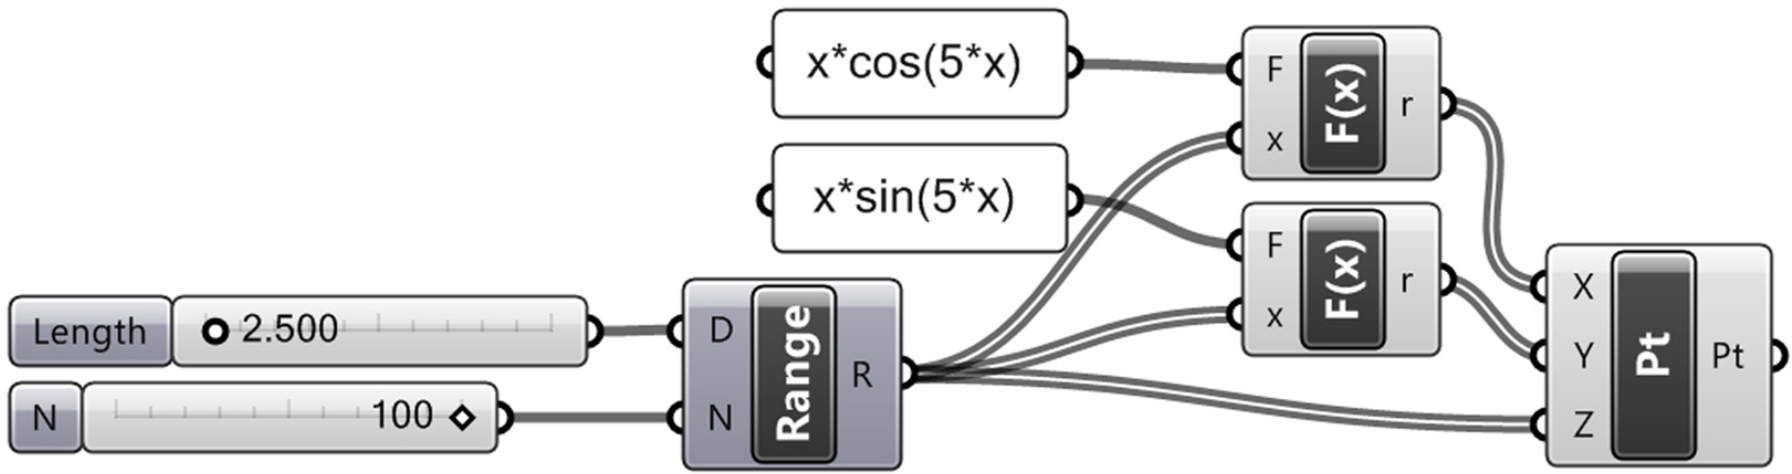
\includegraphics[width=0.8\textwidth]{images/grasshopper}
  %\vspace{-5pt}
    \caption{A program in Grasshopper that computes the 3D coordinates of a conical spiral. Each time the left sliders are dragged a new coordinate is calculated.}
  \label{fig:grass}
  %\vspace{-10pt}
\end{figure}

Like Monkey, Grasshopper is implemented as a \textit{plugin} for Rhino$^{\ref{fnote:rhin}}$. However, Grasshopper tailors the Rhino's environment with specific \gls{gd} tools. These tools are state of the art because they implement important principles for design models, such as the following:

\begin{itemize}
 \item \textit{Get immediate feedback}. As the user interacts with the components, by adding and connecting them, the result reflects immediately in the \gls{cad} model. It facilitates the design conception because the user's intentions are immediately visible. 
 \item \textit{Facilitate program input}. To facilitate the process of design exploration, Grasshopper provides sliders which connect at the component input. Dragging the slider causes a change propagation through components. The components are re-executed with the new slider value. Combined with the above feature new models are generated immediately.
 \item \textit{Correlate the program with the generated elements}. Like DesignScript's watcher, by selecting a component, its geometry is highlighted in the \gls{cad}. It allows designers to understand a program better by figuring out the roles for each element.
 \item \textit{Show comparisons between models}. Grasshopper provides a special component that, when connected to the output of another component, replicates the geometry. This mechanism is useful for design exploration because it maintains in the \gls{cad}'s background an old replica of the changed geometry. It adds a context at each change so that the designer can compare the result of his change in the new geometry based on the old one.
\end{itemize}

Mainly, the Grasshopper interactivity depends on the immediate feedback tool. However, this tool will never scale for arbitrarily complex programs because the \gls{cad}'s render is not designed to process the massive amount of information generated by \gls{gd} methods. Other systems, such as DesignScript and Rosetta, improve this problem by sidestepping most of the functionality of traditional \gls{cad} tools and focusing only on the generation and visualization of geometric models. These systems provide a backend based on OpenGL that is independent of a full-fledged \gls{cad} application, but, in Grasshopper, there is no so backend.

Moreover, the traceability among components is just in one direction. From the designer perspective, it would be more useful start from the geometry and find which component implements it, but it is unsupported. However, despite the usefulness of model comparison in design exploration, this feature is also unsupported.
%%%%%%%%%%%%%%%%%%%%%%%%%%%%%%%%%%%%%%%%%%%%%%%%%%%%%%%%%%%%%%%%%%%%%%%%%%%%%%%%%%%%%%%%%%%%%%%%%%%%%%%%%
\subsection{Dynamo}
\label{subsed:dynamo}
Dynamo\footnote{\texttt{http://dynamobim.com/}} is a programming language and environment designed to support \gls{gd}. Like Grasshopper, Dynamo provides an alternative way to programming. However Dynamo, like DesignScript, is implemented on top of Revit, an Autodesk product for \gls{bim}.

\begin{wrapfigure}{r}{0.5\textwidth}
  %\vspace{-30pt}
  \begin{center}
    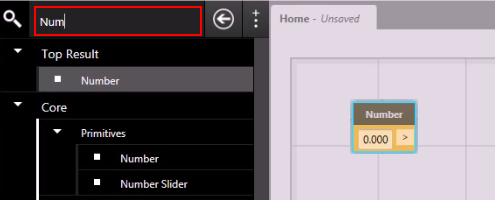
\includegraphics[width=0.5\textwidth]{images/dynam-tab}
  \end{center}
  %\vspace{-18pt}
 \caption{Dynamo search tab. Searching for a component, highlighted in red.}  
  %\vspace{-20pt}
    \label{fig:dynam}
\end{wrapfigure}

Dynamo provides a set of tools similar to Grasshopper, particularly a searching table, as shown in Figure~\ref{fig:dynam}, which provides quick access to the primitives of the language, such as the components and widgets. This feature encourages designers to explore the available parts and try current components.

In general, Dynamo and Grasshopper are programming environments and visual languages popular among novices in programming. The smooth learning curve and perhaps the style of the \gls{ui} elements are attractive for beginners. However as the visual programs become broad and complex, it requires more time to understand, maintain, and adapt to new requirements, than the textual programs as showed in~\citep{leitao2011programming}. Despite spending more time and effort to learn a textual programming language, the learners have their time quickly recovered once the complexity of the design task becomes sufficiently large.
%%%%%%%%%%%%%%%%%%%%%%%%%%%%%%%%%%%%%%%%%%%%%%%%%%%%%%%%%%%%%%%%%%%%%%%%%%%%%%%%%%%%%%%%%%%%%%%%%%%%%%%%%
\subsection{Mathematica}
\label{subsec:mathematica}
Mathematica~\citep{wolfram1991mathematica} is a language and environment built to support scientific calculation. It is widely used in the scientific community, especially by students, because it represents programs using an abbreviated artificial language. This language supports not just direct textual input, but also two-dimensional information, like traditional mathematical notation.

\begin{figure}[!htbp]
%\vspace{-5pt}
  \centering
  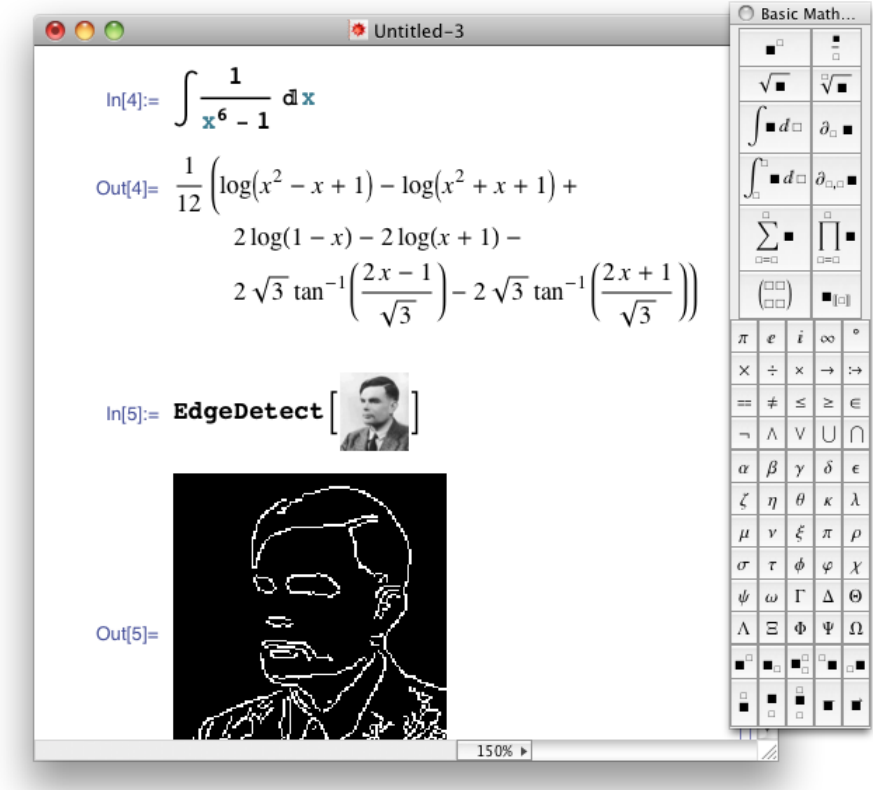
\includegraphics[width=.7\textwidth]{images/mathematica}
  %\vspace{-20pt}
    \caption{Mathematica notebook}  
  \label{fig:math}
  %\vspace{-10pt}
\end{figure} 

The core concepts of Mathematica are based on the paradigm initiated by Turing's work~\citep{wolfram2003wolfram}. In this model, Mathematical processes are systematized as computations. For example, in a typical interaction, the user types a mathematical expression in the Mathematica environment (i.e. notebook), then this expression is evaluated, as shown in Figure~\ref{fig:math}.  

A relevant aspect of Mathematica's notebook is the immediacy that users get a response. Unlike a typical program that must be executed explicitly to get a feedback of an action, in this notebook expressions are evaluated as soon as they are typed. It works like a read-eval-print loop. However, it has enhanced mechanisms to present data meaningfully.

The Mathematica features are well designed to display information in a human readable form. It would be useful for external programming languages if it could take advantage of these functions. Unfortunately, Mathematica is closed for this end.
%%%%%%%%%%%%%%%%%%%%%%%%%%%%%%%%%%%%%%%%%%%%%%%%%%%%%%%%%%%%%%%%%%%%%%%%%%%%%%%%%%%%%%%%%%%%%%%%%%%%%%%%%
\subsection{IPython}
\label{subsec:ipython}

IPython~\citep{PER-GRA:2007} is a programming environment built to support scientific calculation. Unlike Mathematica~\citep{wolfram1991mathematica},  IPython is an open platform for extensions; it allows external programming languages (frontends) to use its features which includes an interactive shell, and a browser-based notebook with support for code, text, mathematical expressions, plots, and other rich media. 

Like Mathematica, IPython has a notebook where users can try out expressions and immediately see its result, as shown in Figure~\ref{fig:ipython}, however, this notebook is in a web format. IPython's architecture is a typical client-server, where the frontend is the client (i.e. the notebook), and the server is a language kernel (i.e. the programming language which users interact with). The communication between client and server is through a strict protocol that the language kernel must implement. 

\begin{figure}[!htbp]
  \centering
    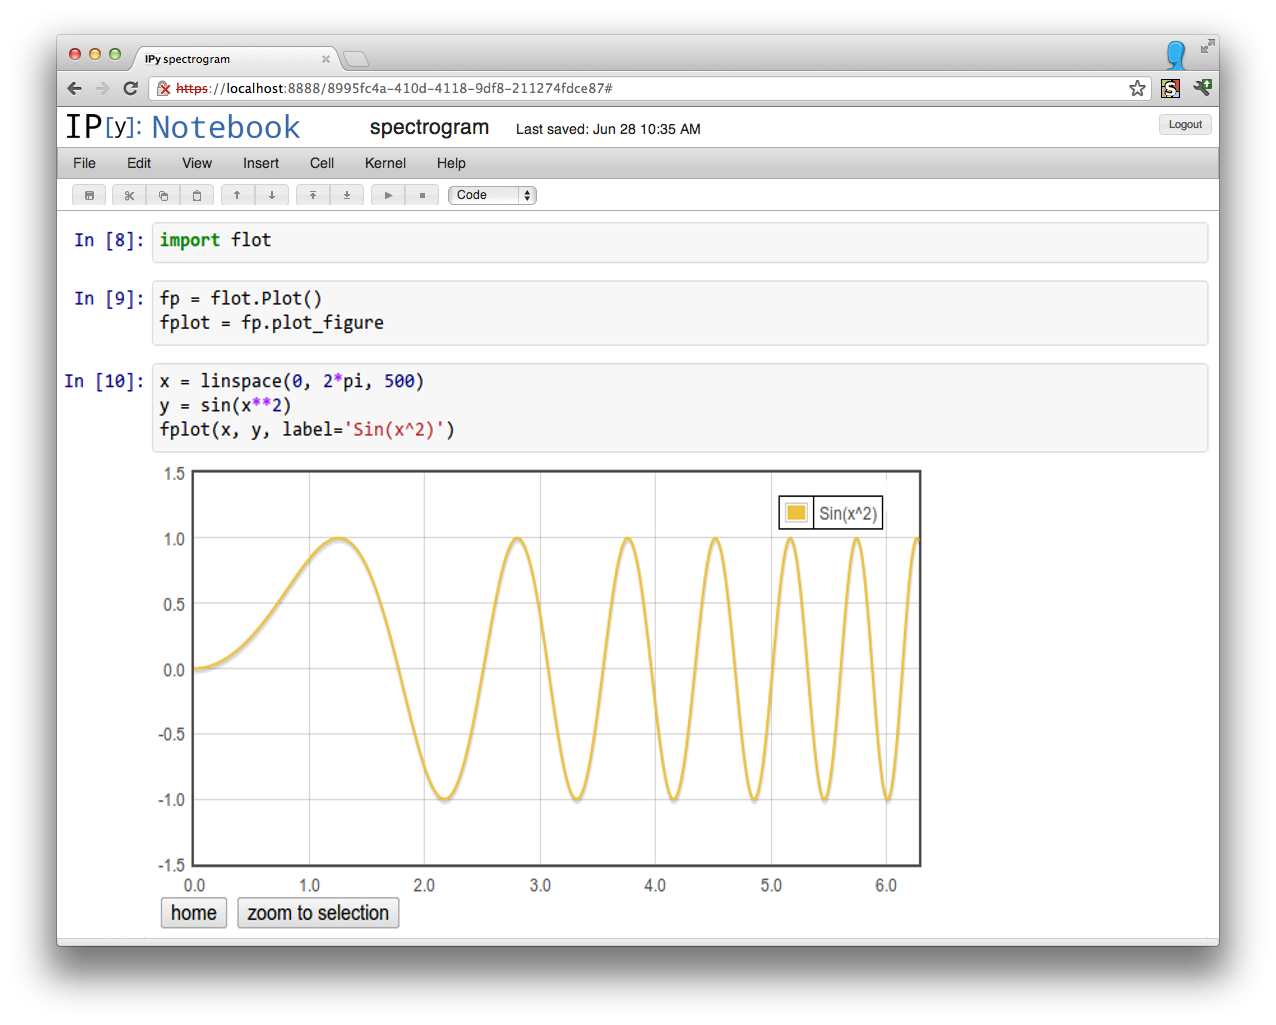
\includegraphics[width=0.7\textwidth]{images/ipython}
 \caption{IPython browser-based notebook}
    \label{fig:ipython}
\end{figure}

IPython provides a base layer for new programming environments, by exposing the major components of its architecture. Consequently, its features are available from other systems. For example, IJulia uses IPython interface with Julia language. 
%%%%%%%%%%%%%%%%%%%%%%%%%%%%%%%%%%%%%%%%%%%%%%%%%%%%%%%%%%%%%%%%%%%%%%%%%%%%%%%%%%%%%%%%%%%%%%%%%%%%%%%%%
\subsection{MathCAD}
\label{subsec:mathcad}
MathCAD\footnote{\texttt{http://www.ptc.com/product/mathcad}} is a programming environment and language built to support scientific calculation. Like Mathematica, MathCAD aims to present information in a human readable form. However, it generates live calculations with graphical plots, text, and images into a single document. This document is the program environment as well as the final product.

The mathematical expressions defined in the MathCAD document act as an associative language. So, when an expression changes its value is propagated through the document. This mechanism is the base of the interactiveness. However, it represents a barrier for program recomposition, because new expressions can change the previous ones. That means that variables have a global scope, the MathCAD document if in somewhere a variable is changed it will be changed in every occurrence in the document.   
%%%%%%%%%%%%%%%%%%%%%%%%%%%%%%%%%%%%%%%%%%%%%%%%%%%%%%%%%%%%%%%%%%%%%%%%%%%%%%%%%%%%%%%%%%%%%%%%%%%%%%%%%             
\section{Summary}

Table~\ref{tab:sum} shows the presented systems based on their major design influences. The table is also intended to address the following questions:

\begin{table}[h]
%\vspace{0pt}
\centering
%\ra{1.0}
\resizebox{\textwidth}{!}{%
\begin{tabular}{@{}clllc@{}}
\toprule
\multicolumn{1}{l}{{\bf Type$^{(1)}$}} & {\bf System} & {\bf Main feature$^{(2)}$} & {\bf \begin{tabular}[c]{@{}l@{}}Support to understand \\ programs$^{(3)}$\end{tabular}} & {\bf Representation of code$^{(4)}$} \\ \midrule
\multirow{6}{*}{GS} & Eclipse & \multirow{4}{*}{\begin{tabular}[c]{@{}l@{}}support software \\ development life cycle\end{tabular}} & \multirow{4}{*}{debugger} & \multirow{16}{*}{text} \\
 & NetBeans &  &  &  \\
 & IntelliJ &  &  &  \\
 & MVS &  &  &  \\ \cmidrule(lr){2-4}
 & Xcode & \multirow{2}{*}{observable programming} & \multirow{2}{*}{live execution feedback} &  \\
 & LightTable &  &  &  \\ \cmidrule(r){1-4}
\multirow{7}{*}{TS} & LOGO & \multirow{2}{*}{understandable language} & \multirow{2}{*}{physical interpretation} &  \\
 & SmallTalk &  &  &  \\ \cmidrule(lr){2-4}
 & Processing & \multirow{2}{*}{visual context} & \multirow{2}{*}{instant visualization} &  \\
 & Fluxus &  &  &  \\ \cmidrule(lr){2-4}
 & DrRacket & gradual learning & debugger; stepper &  \\ \cmidrule(lr){2-4}
 & PythonTutor & \multirow{2}{*}{show program flow} & \multirow{2}{*}{\begin{tabular}[c]{@{}l@{}}navigate through the \\ program execution\end{tabular}} &  \\
 & YinYang &  &  &  \\ \cmidrule(r){1-4}
\multirow{8}{*}{ES} & DesignScript & \multirow{3}{*}{\begin{tabular}[c]{@{}l@{}}support generative design \\ methods\end{tabular}} & \multirow{3}{*}{debugger} &  \\
 & Monkey &  &  &  \\
 & Rosetta &  &  &  \\ \cmidrule(l){2-5} 
 & Grasshopper & \multirow{2}{*}{\begin{tabular}[c]{@{}l@{}}alternative way to \\ expressing programs\end{tabular}} & \multirow{2}{*}{dataflow paradigm} & \multicolumn{1}{l}{\multirow{2}{*}{graphical components}} \\
 & Dynamo &  &  & \multicolumn{1}{l}{} \\ \cmidrule(l){2-5} 
 & Mathematica & \multirow{3}{*}{\begin{tabular}[c]{@{}l@{}}support scientific \\ calculation\end{tabular}} & \multirow{3}{*}{present data meaningfully} & \multicolumn{1}{l}{\multirow{3}{*}{mathematical forms}} \\
 & IPython &  &  & \multicolumn{1}{l}{} \\
 & MathCAD &  &  & \multicolumn{1}{l}{} \\ \bottomrule
\end{tabular}
}
%\vspace{1pt}
\caption{System attributes}
%\vspace{-20pt}
\label{tab:sum}
\end{table}

(1) \textit{What is the purpose of the system?} We categorized three main goals for a system. \gls{gs} designed for building complex software for the industry; \gls{ts} designed to help people learn how to program; \gls{es} designed to help people create things that are tailored to their needs.

(2) \textit{How does the system support its purpose?} We identified the following strategies: (i) support software development life cycle, (ii) turn programming in something more observable, (iii) create an understandable language, (iv) combine textual programming with a visual context, (v) support gradual learning in a single environment, (vi) show the program flow, (vii) support generative design methods, (viii) find alternative ways for to express programs, and (ix) support scientific calculation.

(3) \textit{Does the programming environment provide additional assistance to enable users to understand the behavior of their programs better?} Environments in our study used several techniques to help users understand the behavior of their programs. These included (i) a debugger which contributes to find bugs in the program, (ii) an enhanced debugger which provides live execution feedback, (iii) languages with strong metaphor allowing physical interpretation, (iv) instant visualization of models, (v) navigation through the program's execution (vi) assembling components in a dataflow paradigm and (vii) present data adequately.

(4) \textit{How does code look in the programming environment or language?} The systems in our study represent programs using text, users can type, graphical components, users can manipulate, and mathematical forms users can fill in.

\section{Conclusion}

In the surveyed systems, the typical representation of code is textual. This representation is typically static and, to be understood, requires the reader to know the vocabulary of the programming language. For a novice, it is simply a barrier to learning. On the other hand, the representation of programs as graphical components or mathematical forms lowers this barrier, because the information is visually more perceptible, but it becomes incomprehensible as the program grows.